\documentclass[12pt]{HomusWorkus}

% \usepackage[Hhtbp]{algorithm2e}
\usepackage{listings}

\begin{document}

% ------------------------------------------------------------
%           Титульна сторінка
% ------------------------------------------------------------
\begin{titlepage}
    % \begin{figure}
    %     \centering
    %     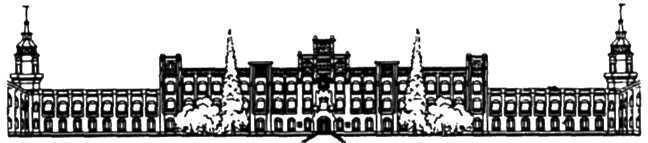
\includegraphics[scale=0.6]{Images/kpi_1.png}
    % \end{figure}

    \begin{center}
        \small{\textbf{НАЦІОНАЛЬНИЙ ТЕХНІЧНИЙ УНІВЕРСИТЕТ УКРАЇНИ\\
        «КИЇВСЬКИЙ ПОЛІТЕХНІЧНИЙ ІНСТИТУТ імені ІГОРЯ СІКОРСЬКОГО»\\
        НАВЧАЛЬНО-НАУКОВИЙ ФІЗИКО-ТЕХНІЧНИЙ ІНСТИТУТ\\
        }}
        
        \vfill
        \Huge{\textbf{СУЧАСНI АЛГЕБРАЇЧНI КРИПТОСИСТЕМИ}}

        \vspace{0.2cm}
        \large{\textbf{КОМП’ЮТЕРНИЙ ПРАКТИКУМ}}

        \vspace{0.2cm}
        \large{\textit{
            Дослiдження сучасних алгебраїчних криптосистем
        }}
        
        % \vspace{0.2cm}
        % \large{\textbf{Варіант 1}}

        \vfill
        \large{
            \begin{flushright}
                \begin{tabular}{l}
                    \hskip-0.5cm \textbf{Виконали:}  \\
                    Волинець Сергій ФІ-42мн \\
                    Сковрон Роман ФІ-42мн \\
                    % \hskip-0.5cm \textbf{Перевірив:}  \\
                    % Волинець Сергій ФІ-03  \\
                \end{tabular}
            \end{flushright}
        }

        \vfill
        \large{Київ --- \the\year{}}
    \end{center}
\end{titlepage}
\addtocounter{page}{1}

% ------------------------------------------------------------
%           Зміст
% ------------------------------------------------------------
\tableofcontents
\newpage

% ------------------------------------------------------------
%           Основний текст
% ------------------------------------------------------------

\section{Мета проведення комп’ютерного практикуму}

Дослiдження особливостей реалiзацiї сучасних алгебраїчних криптосистем на прикладi
учасникiв першого раунду процесу стандартизацiї постквантової криптографiї (NIST PQC).

\section{Постановка задачi}

Розробити програмну реалiзацiю обраного криптографiчного алгоритму. Реалiзацiя повинна мiстити всi можливi варiанти алгоритму. Коректнiсть реалiзацiї пiдтвердити за допомогою тестiв, якi використовують за наявностi офiцiйнi тестовi вектори або офiцiйну реалiзацiю. Знайти схожi алгоритми та провести порiвняльний аналiз швидкодiї за рiзних умов та використання модифiкацiй складових частин. Навести повний теоретичний опис алгоритму з усiма деталями та вiдомими результатами дослiджень. Провести теоретичний порiвняльний аналiз обраного алгоритму зi схожими алгоритмами та дослiдити можливiсть перенесення вiдомих атак на обраний алгоритм.

\section{Хiд виконання роботи, опис труднощiв, що виникали, та шляхи їх подолання}

Хід виконання роботи почався з вибору криптографічного алгоритму для розробки програмної реалізації. Обравши алгоритм цифрового підпису CRYSTALS-Dilithium, було проведено детальний теоретичний аналіз принципів його роботи та механізмів безпеки, що закладені в алгоритмі. Далі, було реалізовано всі можливі варіанти алгоритму, а саме спрощену, та розширену версії. Окрім того, варти уваги той факт, що алгоритми, можуть мати екілька рівнів безпеки, в залежності від значення глобальних змінних.

Під час розробки виникли деякі труднощі, зокрема, з оптимізацією швидкодії алгоритму для різних умов та для різних обсягів даних. Для вирішення цих проблем було досліджено еталонну реалізацію наведену в документації, разом з описом.

\section{Опис обраного криптографiчного алгоритму та його складових частин}

Алгоритм підпису Dilithium є частиною класу постквантових криптографічних алгоритмів, що забезпечує цифрові підписи з високим рівнем безпеки. В його основі лежать такі примітиви, як множення матриць, бітові та байтові операції, тощо. Основні складові частини, що описані в протоколі до алгоритму, це генерація ключів, підписування та перевірка підпису.

На початку генерується секретний ключ і публічний ключ. Секретний ключ включає випадкові значення, які генеруються з використанням сід-значень $\rho$ і $K$. Публічний ключ $\mathbf{t}$ обчислюється як результат множення матриці $\mathbf{A}$ на вектор $\mathbf{s_1}$, після чого застосовується функція $\mathrm{Power2Round}$ для створення зменшеного представлення. Таким чином, публічний ключ містить значення $\mathbf{t_1}$, яке використовуватиметься в наступних етапах підписування та перевірки.

Для створення підпису, підписувач використовує секретний ключ і повідомлення $M$, для якого обчислюється його хеш $\mu$. Потім генерується маска для випадкових чисел, що використовується в процесі підпису. Підпис складається з двох частин: вектора $\mathbf{z}$ і допоміжної інформації $\mathbf{h}$, яка містить позиції переповнень у підписі, і контрольного значення $c$, яке використовується для підтвердження дійсності підпису. Щоб уникнути використання чисто випадкових значень для підпису використовується геш функція SHAKE-256, що дозволяє ортимати геш значення довільної довжини.

Під час перевірки підпису за допомогою публічного ключа $\mathbf{t_1}$ і повідомлення $M$ перевіряється правильність обчислень, а саме: чи співпадають контрольні значення та чи відповідає підпис заданим критеріям. Процес верифікації включає перевірку переповнень у векторі $c\mathbf{t_0}$ і коректність хешування, щоб забезпечити, що підпис не був підроблений.

Проблеми можуть виникати через необхідність значної кількості обчислень, особливо при створенні та перевірці підписів. Для оптимізації використовується спеціалізоване представлення матриць у вигляді NTT (Number Theoretic Transform), що дозволяє значно зменшити обсяг обчислень, необхідних для множення матриць і хешування. Однак, зменшення розміру публічного ключа за рахунок відкидання деяких коефіцієнтів може ускладнити перевірку підпису, оскільки потрібна додаткова інформація про позиції переповнень, яка передається у вигляді допоміжних даних в підписі.

Таким чином, кожен з етапів алгоритму — від генерації ключів до підписування та перевірки підпису — має свої виклики, пов'язані з оптимізацією швидкості, збереженням пам'яті та забезпеченням високого рівня безпеки. Алгоритм Dilithium вирішує ці проблеми через використання ефективних математичних інструментів, зокрема NTT.

\section{Порiвняльний аналiз швидкодiї обраного алгоритму зi схожими алгоритмами}

Алгоритм підпису Dilithium був розроблений як одна з найбільш ефективних постквантових схем підпису, що поєднує хорошу швидкодію та оптимізацію для зменшення розмірів публічних ключів і підписів. Щоб порівняти його з іншими алгоритмами постквантового підпису, важливо розглянути ключові параметри: розміри підпису та публічного ключа, швидкість підписування та перевірки, а також складність реалізації.

Однією з основних переваг Dilithium є використання операцій NTT (Number Theoretic Transform), що дозволяє значно прискорити операції множення поліномів порівняно з іншими методами, такими як прямі множення. Для оптимізації цих операцій Dilithium пропонує використовувати цілісні арифметичні операції на процесорах з підтримкою AVX2. В порівнянні з іншими постквантовими схемами, такими як NTRU або NTS, які вимагають використання гауссового вибірки, що є складнішим і повільнішим процесом, Dilithium показує кращу швидкодію, оскільки він використовує лише рівномірний розподіл, що значно зменшує складність реалізації та тестування. Середній час підписування для Dilithium в два рази швидший за схеми на основі NTRU, а перевірка підпису займає менше часу завдяки зменшеному розміру публічного ключа і використанню ефективних трансформацій.

У порівнянні з іншими криптографічними схемами, Dilithium має середній розмір підпису близько 2.7KB, що є більшим за деякі альтернативи, такі як схеми на основі багаточленових підписів, де підпис може бути меншим за 100 байт. Однак у порівнянні з іншими лінійними схемами підпису на основі решіток (наприклад, NTRU), де підписи можуть досягати 1.5KB, Dilithium пропонує найкращий баланс між розміром і швидкодією. Крім того, публічні ключі в Dilithium мають розмір, який також зменшено завдяки оптимізації параметрів, зокрема розміру коефіцієнтів у публічному ключі. У схемах, таких як Ring-LWE або Multivariate підписи, публічні ключі можуть бути значно більшими, що знижує ефективність їх використання в системах з обмеженими ресурсами.

У порівнянні з хешованими підписами, які мають невеликі публічні ключі (менше 100 байт), але значно більші підписи (30-40KB), Dilithium пропонує значно кращу швидкість підписування, що в середньому в 50 разів швидше. Інші схеми, такі як Multivariate Signature Schemes, можуть мати ще менші підписи, але потребують значно більших публічних ключів (понад 100KB) і часто мають меншу ефективність через велику кількість обчислень, необхідних для їх створення.

Загалом, Dilithium виділяється завдяки оптимальному балансу між швидкістю, розмірами ключів та підписів, що робить його потужним кандидатом для широкого використання в постквантових криптографічних системах.

\section{Огляд наявних результатiв дослiджень обраного алгоритму}

У дослідженнях самих авторів, що стосуються алгоритму Dilithium, важливу роль відіграє редукція ґратки та її зв'язок з розв'язуванням задачі пошуку короткого вектора в ґратці (SVP). Основним методом для знаходження коротких векторів у Евклідових ґратках є алгоритм BKZ (Block-Korkine-Zolotarev), який застосовує розв'язок задачі SVP для блоків розміром $b$. Безпека схеми Dilithium базується на складності вирішення задачі SVP для великих розмірів блоків $b$, оскільки час виконання класичних і квантових рішень цієї задачі є експоненційним відносно $b$. Найкращі відомі алгоритми для вирішення задачі SVP на класичних та квантових комп'ютерах мають складність порядку $2^{c_C b}$, де $c$ є константами для класичних $(c_C \approx 0.292)$ та квантових рішень $(c_Q \approx 0.265)$. Тому зміна розміру блоку $b$ без суттєвого прориву в теорії не дозволить значно зменшити складність.

Щодо алгебраїчних атак на систему Dilithium, дослідження показують, що використовувані параметри є стійкими до основних типів атак, таких як прямі та дуальні атаки на основі матриць LWE (Learning With Errors). Крім того, алгебраїчні атаки на криптографічні схеми, такі як Ring-LWE, менш ефективні в разі використання Multivariate LWE (MLWE), що віддаляє систему від слабких структур на решітках. Навіть атаки, засновані на пошуку коротких векторів за допомогою алгоритмів BKZ, не дають суттєвих переваг без використання дуже великих параметрів блоку $b$. Враховуючи ці аспекти, атаки на схему Dilithium виявляються малоймовірними за умови належно налаштованих параметрів.

% \section{Результати порiвняльного аналiзу стiйкостi обраного алгоритму зi схожими алгоритмами з обґрунтуванням можливостi застосування вiдомих атак}

\section{Опис власних тестiв, якi проводилися з метою перевiрки коректностi реалiзованої програми}

Для проведення тестів, було переглянуто яким чином перевіряється коректність еталонної імплементації. В результаті, було визначено, що автори один раз виконують підписування та перевірку, для одного повідомлення, з подальшим заміром швидкодії кожного з трьох основних алгоритмів.
Для наочності, результати швидкодії еталонної реалізації наведені в таблиці \ref{tab:speeeeed} разом з замірами нашої реалізації спрощеної схеми. Для більш точних оцінок, було проведено заміри на 100 випадкових текстах. 

\begin{table}[ht]
    \centering
    \begin{tabular}{|c|c|c|}
        \hline
        Алгоритм & Еталонна розширена реалізація & Наша спрощена реалізація \\\hline
        $\mathrm{GEN}$ & 0.05696 мс & 6.1304 с \\\hline
        $\mathrm{Sign}$ & 0.3186 мс & 15.0656 с \\\hline
        $\mathrm{Verify}$ & 0.06625 мс & 3.8037 с \\\hline
        \hline
    \end{tabular}
    \caption{Результати дослідження швидкодії}
    \label{tab:speeeeed}
\end{table}

Разом із замірами швидкодії, проводилися заміри коректності. В результаті, було визначено, що алгоритм працює правильно.
Нажаль, заміри для розширеної реалізації не вдалося провести, в наслідок того, що створена реалізація містить недоліки, які перешкоджають створенню правильного підпису. Ця проблема була виявлена при перевірці коректності.


\section{Детальний опис особливостей реалiзацiї та приклади застосування}

При реалізації та дослідженні еталонної імплементації, було виявлено, що деякі змінні є глобальними та постійними, а отже немає потреби передавати їх в кожну функцію по ланцюжку, що збільшує зрозумілість коду. Основними реалізованими алгоритмами є такі алгоритми як $\mathrm{Gen}$, $\mathrm{Sign}$, $\mathrm{Verify}$. Для їх роботи було реалізовано додаткові алгоритми:
\begin{enumerate}
    \item matrix\_mul, matrix\_const\_mul, matrix\_sum, matrix\_sub -- для операцій з матрицями поліномів, таких як множення, множення на константу, додавання і віднімання.
    \item modpm -- реалізує операцію $a \mod^{\pm} q$.
    \item random\_polynomial\_Zq -- генерує випадковий многочлен з коефіцієнтами, обраними з скінченного поля $\mathbb{Z}_q$. Залежно від заданих параметрів, коефіцієнти створеного полінома можуть бути обмежені деяким малим значенням для обмеження шуму.
    \item Norm\_polyvec, Norm\_polyvec\_check, Norm\_matr ,  Norm\_matr\_check
    \item decompose, HighBits, LowBits -- використовуються для розкладання заданого значення за модулем $Q$ на дві складові, $r_1$ і $r_0$.
\end{enumerate}

Як приклад застосування можна розглянути наступний код, що знаходить підпис до двох повідомлень і перевіряє їх.

\begin{lstlisting}[language=Python]
    print("Key generation...")
    pk, sk = Gen()
    print("Key is generated")
    print("")
    
    M1 = "Some text1"
    M2 = "Some text2"
    print("Sign first message...")
    sigma1 = Sign(sk=sk, M=M1)
    print("Sign second message...")
    sigma2 = Sign(sk=sk, M=M2)
    print("Messages are signed...")
    print("")
    
    print("Verify signature of the messages")
    print(f"First signature correctness:", Verify(pk=pk, M=M1, sigma=sigma1))
    print(f"Seccond signature correctness:", Verify(pk=pk, M=M2, sigma=sigma2))
    print("")
\end{lstlisting}

\section{Результати аналiзу постквантової стiйкостi за наявними результатами аналiзу}

Наявний аналіз показує, що навіть за умов розвитку квантових алгоритмів, такі схеми залишаються стійкими до атак з використанням квантових обчислень. Алгоритм BKZ, який використовує блокове зменшення решітки, демонструє потужність у зменшенні довжини векторів у решітках, але для досягнення справжнього прориву в швидкості вирішення задачі SVP (Shortest Vector Problem) ще далеко. Квантові алгоритми, хоч і дають деяке покращення (наприклад, зменшення часу розв'язання задачі SVP), не здатні значно перевищити класичні методи на даному етапі розвитку технологій. Крім того, деякі види атак, зокрема BKW та Arora-Ge, не є конкурентоспроможними проти новітніх схем на основі MLWE (Modified Learning With Errors). Переходячи від Ring-LWE до MLWE, криптографічні конструкції віддаляються від слабких алгебраїчних властивостей, що робить їх менш уразливими до алгебраїчних атак. Оскільки такі криптосистеми на основі решіток не мають суттєвих вразливостей, навіть в умовах потужних квантових атак, вони виглядають перспективними для використання в постквантових криптографічних додатках.


\section{Висновки до роботи}

У процесі виконання роботи було реалізовано криптографічний алгоритм цифрового підпису CRYSTALS-Dilithium, що є частиною постквантових криптосистем, і проведено детальний теоретичний аналіз його принципів і механізмів безпеки. Було розглянуто різні варіанти реалізації алгоритму, включаючи спрощену і розширену версії, а також виконано оптимізацію швидкодії для різних обсягів даних. Під час розробки виникли труднощі, зокрема, при оптимізації швидкодії. Результати тестів підтвердили коректність реалізації алгоритму, хоча були зафіксовані проблеми з розширеною реалізацією через недоліки в коді.

Порівняльний аналіз показав, що Dilithium ефективно поєднує хорошу швидкодію та оптимізацію розміру публічних ключів і підписів, що робить його одним із найкращих кандидатів для постквантових криптосистем. Завдяки використанню операцій NTT (Number Theoretic Transform), цей алгоритм показує значно кращу швидкість підписування та перевірки, ніж альтернативи, такі як NTRU, а також забезпечує високий рівень безпеки завдяки складності задачі пошуку короткого вектора у ґратці.




% % ------------------------------------------------------------
% %           Bibliography
% % ------------------------------------------------------------
% \bibliographystyle{alpha}
% \bibliography{sample}

\end{document}
